\section{Introdução}

\subsection{Contexto}
\begin{frame}
	\begin{itemize}
		\item Aumento da presença de serviços digitais na vida cotidiana;
		\item Acumular dados não é o suficiente;
		\item Métodos tradicionais de análise estatística requerem interpretação manual;
		\item Fayyad (1996) \cite{fayyad1996} diz que neste cenário há uma grande necessidade de novas teorias e ferramentas computacionais a fim de auxiliar na extração de conhecimento dos grandes e cada vez maiores volumes de dados.
	\end{itemize}
\end{frame}

\subsection{Processo de KDD}

\begin{frame}
	\begin{itemize}
		\item Knowledge Discovery in Databases - cunhado por Shapiro em 1989;
		\item Processo iterativo e não trivial dependente de interações do usuário;
		\item Tem como objetivo identificar informações válidas, novas, potencialmente úteis e compreensíveis em um grupo de dados.
	\end{itemize}
\end{frame}

\begin{frame}
	\begin{figure}[h!]
		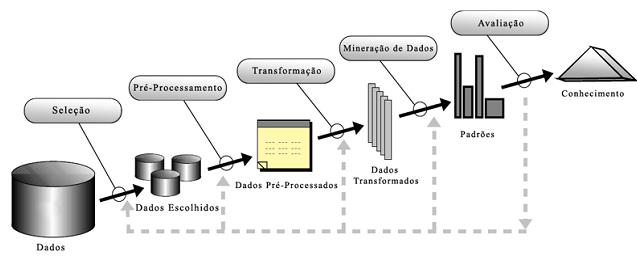
\includegraphics[width=\textwidth]{KDD}
		\caption{Fluxograma do processo de KDD. Adaptado de Fayyad (1996) \cite{fayyad1996}.}
	\end{figure}
\end{frame}

\begin{frame}
	\begin{itemize}
		\item A mineração de dados é uma das etapas do KDD que mais recebe destaque;
		\item Grande quantidade de técnicas e resultados disponíveis para teste;
		\item Descoberta e adaptação de padrões e modelos;
		\item Classificação, Clusterização e Regressão.
	\end{itemize}
\end{frame}